\section{Gestione delle Risorse}

Come visto precedentemente uno dei compiti più importanti del sistema operativo è la gestione delle risorse di sistema, come la memoria, i dispositivi I/O, ecc..

\subsection{Gestione dei Processi}
Un programma è un'entità "passiva", memorizzata sul disco, mentre il processo è "attivo".
I programmi dientano processi quando vengono caricati in memoria principale.

\subsubsection*{Stato del processo}
\begin{itemize}
    \item \textbf{New:} il processo viene creato, diventerà ready appena il sistema operativo lo inserirà nella ready queue.
    \item \textbf{Ready:} il processo risiede in memoria principale ed è in attesa di essere assegnato ad un processore.
    \item \textbf{Running:} Vengno eseguite le istruzioni del processo, i processi vengono selezionati dal dispatcher tra quelli nella ready queue e ci possono ritornano nel caso in cui lo scheduler trovi un processo più importante oppure per un interrupt esterno.
    \item \textbf{Waiting:} il processo è in attesa di un evento, questo avviene da parte del processo stesso nel caso di una richiesta ad un dispositivo I/O
    \item \textbf{Terminated:} il processo ha terminato la propria esecuzione. Può essere dovuto dal processo che ha terminato (o ricevuto un errore), oppure può essere dettato dal sistema operativo per un utilizzo scorretto delle risorse.
\end{itemize}

\begin{figure}[H]
    \centering
    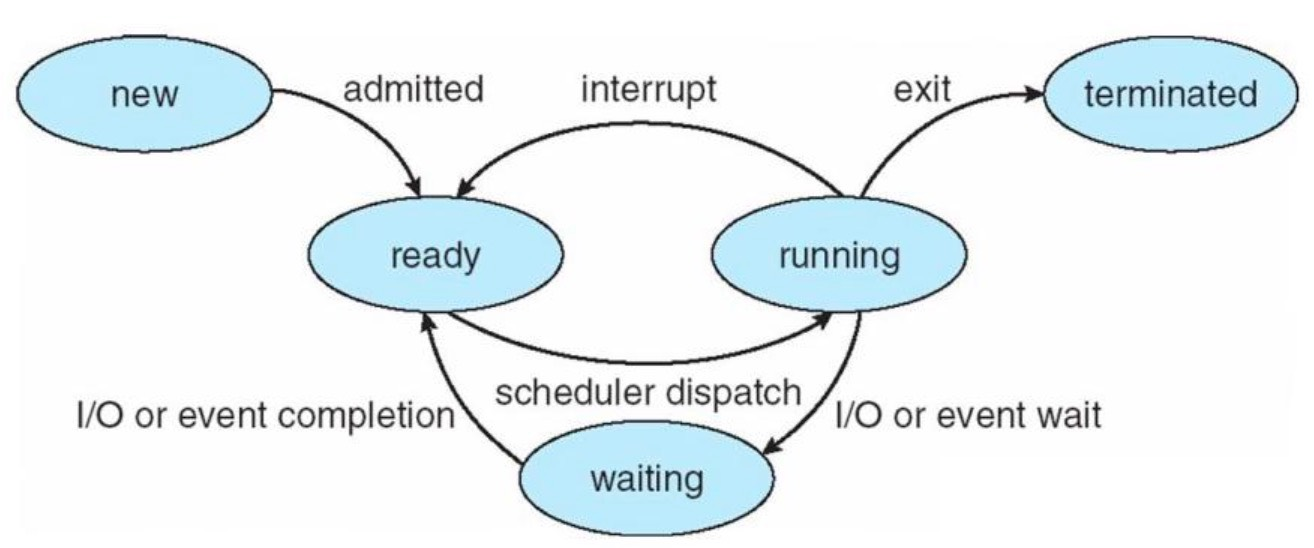
\includegraphics[width=0.6\linewidth]{assets/process.jpg}
    \caption{Process lifecycle}
\end{figure}

\subsubsection*{Informazioni del processo}
\begin{sitemize}
    \item \textbf{Informazioni sul processo} quali stato, priorità e numero identificativo.
    \item Una \textbf{sezione di testo} dove è contenuto il codice del programma da
    eseguire.
    \item Il \textbf{program counter}, l'indirizzo di memoria della prossima istruzione da eseguire ed il \textbf{contenuto dei registri} della CPU.
    \item Lo \textbf{stack}, ovvero i dati temporanei, parametri per i sottoprogrammi, indirizzi di rientro e variabili locali.
    \item Una \textbf{sezione dati}, le variabili globali.
    \item Un \textbf{heap}, memoria dinamicamente allocata durante l'esecuzione del task.
    \item Informazioni sulla \textbf{contabilizzazione} delle risorse (tempo di utilizzo della CPU, ecc... ).
\end{sitemize}

\spacer
Queste informazioni, o i riferimenti a tali informazioni vengono salvati nel \textit{Process Control Block} (PCB), che a sua volta è salvata nella tabella dei processi.

\begin{note}
    Un programma non ha necessariamente un solo processo, ma esso descrive un insieme di processi.
\end{note}

\subsubsection{Threads}
Un processo deve sempre avere almeno un thread (sè stesso), ma può generarne altri in caso abbia bisogno di eseguire delle operazioni simultaneamente sfruttando il multithreading.

\spacer
Tutti i thread di un processo condividono le risorse che sono state assegnate al processo, risiedono nello stesso spazio di indirizzamento e hanno accesso agli stessi dati.

Ogni thread ha un program counter, uno stato, uno spazio di memoria, uno stack e un descrittore.

\spacer
Un processore dotato di Hyper-Threading può eseguire 2 thread contemporaneamente, è in grado di eseguire più istruzioni su dati separati in parallelo.

\subsubsection{Multiprogrammazione e Multitasking}
La multiprogrammazione è un aspetto fondamentale di un sistema operativo. Infatti un singolo processo non è in grado di mantenere sempre occupata la CPU, inoltre spesso gli utenti vogliono essere in grado di eseguire più programmi contemporaneamente.

\spacer
Il sistema memorizza più processi nella memoria principale rendendo possibile così lo switching tra un contesto ed un'altro. Uno specifico algoritmo di scheduling ha il compito di decidere quando e come effettuare questo switch.

\spacer
La multiprogrammazione rende possibile il multitasking, dove il sistema cambia velocemente da un processo all'altro al punto che all'utente sembra che non ci siano interruzioni.

\subsection{Gestione della Memoria}
La memoria centrale ha un'importanza centrale nell'architettura di Von Neumann ed è l'unica memoria di grandi dimensioni a cui la CPU ha accesso diretto (accedere al disco richiede un'operazione di I/O)

\spacer
Il Sistema operativo, rispetto alla memoria principale, ha il compito di:
\begin{sitemize}
    \item Tener traccia di quali parti sono utilizzate e da chi.
    \item Decidere quali processi caricare in memoria quando c'è dello spazio disponibile.
    \item Allocare e deallocare spazio di memoria secondo necessità.
\end{sitemize}

\spacer
Il sistema operativo è anche responsabile di gestire in modo efficiente la memoria secondaria, in quanto spesso non è possibile caricare l'intero programma in memoria principale

\begin{figure}[H]
    \centering
    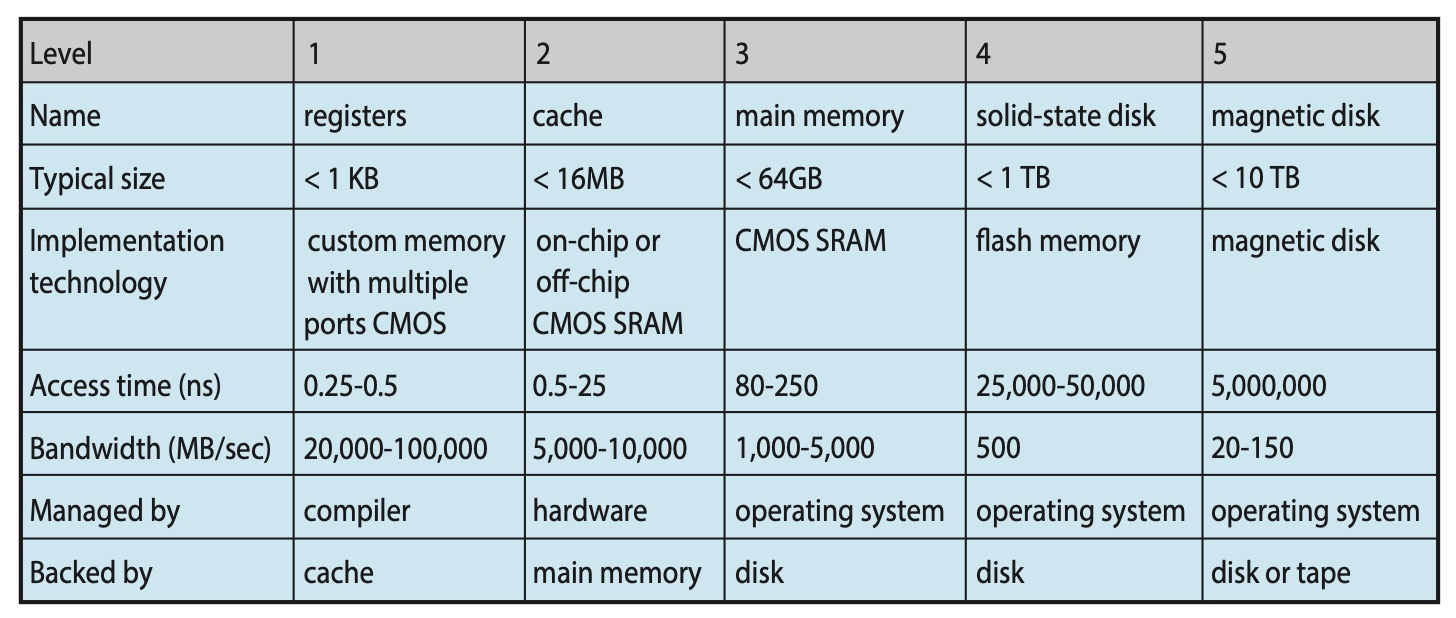
\includegraphics[width=0.75\linewidth]{assets/memory-size.jpg}
\end{figure}

\begin{note}
    Inoltre bisogna considerare che, sopratutto nei sistemi multiprocessore, l'aggiornamento di un dato deve essere riflesso non solo nel file in cui risiede, ma anche in memoria principale e nelle cache degli altri dispositivi.
\end{note}

\subsubsection{File System}
Un file è una \textbf{collezione di informazioni} correlate contenenti dati e programmi.

I file vengono organizzati dal file system in directory, questo permette di effettuare controlli di accesso per verificare che l'utente abbia accesso a quelle risorse.

\spacer
Il sitema operativo è responsabile delle seguenti attività per la gestione di file:
\begin{sitemize}
    \item Creazione e cancellazione di file e directory
    \item Supporto alle funzioni elementari per la manipolazione di file e directory
    \item Associazione dei file ai dispositivi di memoria secondaria
    \item Backup di file su dispositivi stabili di memorizzazione
\end{sitemize}

\subsection{Strutture Dati del Kernel}
Un argomento centrale all'implementazione di un sistema operativo sono le strutture dati, qui vengono descritte le strutture dati utili per la costruzione di sistemi operativi.
Le strutture dati vengono qui solo citate in quanto sono state già approfondite nel corso di Dati e Algoritmi.

\subsubsection{Liste, Pile e Code}
La struttura dati più comune per implementare le liste sono le liste concatenate (standard, doppiamente concatenate e circolari).

Le liste vengono spesso utilizzate per implementare Pile (implementate con politica LIFO) e Code (con politica FIFO).
In particolare la Pila viene utilizzata per implementare lo Stack, utilizzato in diverse situazioni nel sistema operativo.

\subsubsection{Alberi}
Sono utilizzati per rappresentare la relazione causale padre-figlio oppure per implementare degli algoritmi di ricerca binaria efficienti.

\subsubsection{Hashtable}
Vengono utilizzate per memorizzare insiemi di dati con la possibilità di reperire un qualsiasi elemento con una complessità in tempo pari (o quasi) a $O(1)$

\spacer
Le funzioni di hashing banali soffrono del problema del "paradosso del compleanno".
Ovvero in un gruppo di 23 persone la probabilità che 2 di esse compia gli anni lo stesso giorno è >50\%, questo significa che se su una tabella di 365 elementi si inseriscono più di 23 elementi allora c'è una probabilità >50\% di una collisione.
